\documentclass[bigger]{beamer}
%\documentclass[handout]{beamer}
\setbeamertemplate{bibliography item}{}
\usepackage[utf8]{inputenc}
\usepackage[english]{babel}
\usepackage{multirow}
\usepackage{synttree}
\usepackage{booktabs}
\usepackage[backend=bibtex,natbib,style=authoryear]{biblatex}
\usetheme{Warsaw}
%\usefonttheme[onlylarge]{structuresmallcapsserif}
\newcommand{\wigegraph}[1]{\begin{figure}[h]
\centering\includegraphics[width=\textwidth]{#1}\end{figure}}
% Ez most valamiert besz.rt, ugyhogy kikommentalom:
%\AtBeginSection[]{\frame{\frametitle{Outline}\tableofcontents[current]}}

\AtBeginPart{\frame{\partpage}} 

\usepackage{tikz}
\usepackage{tikz-qtree}
\usepackage{xspace}

\bibliography{ml}

\newcommand{\defl}{\texttt{dep\_to\_4lang}\xspace}
\newcommand{\difl}{\texttt{dict\_to\_4lang}\xspace}
\newcommand{\tfl}{\texttt{text\_to\_4lang}\xspace}
\newcommand{\tefl}{\texttt{text\_to\_4lang}\xspace}
\newcommand{\fl}{\texttt{4lang}\xspace}

\newcommand{\edge}[3]{\texttt{#1}~$\xrightarrow#2$~\texttt{#3}}
\newcommand{\twoedges}[4]{\texttt{#1}~$\overset{#2}{\underset{#3}{\rightleftharpoons}}$~\texttt{#4}}
\newcommand{\bin}[3]{
    \texttt{#2}~$\xleftarrow1$~\texttt{#1}~$\xrightarrow2$~\texttt{#3}}

\newcommand{\todo}[1]{\textbf{TODO: #1}}

%\usepackage{apacite}
%\let\cite\shortcite  % to get "et al." for more than two authors
%\let\citeA\shortciteA
\begin{document}

\title{Szemantikai elemz\'es gr\'af-transzform\'aci\'okkal}
\author{Kov\'acs \'Ad\'am \\ G\'emes Kinga}
\institute{Automatizálási és Alkalmazott Informatikai Tanszék \\
Budapesti Műszaki és Gazdaságtudományi Egyetem \\
\texttt{adaam.ko@gmail.com}, \texttt{kinga.andrea.gemes@gmail.com}}

\date{Tudományos Diákköri Konferencia\\2018.11.14.}

%-----------------------

\begin{frame} 

\titlepage 

\end{frame} 

%-----------------------
%-----------------------

\begin{frame} 

    \frametitle{Kontribúciónk} 
    \begin{itemize}
        \pause \item Gráf alapú szemantikai modellek definiálása
        \pause \item Automatizált metódus nyers szöveg szemantikai elemzésére
        \pause \item Modelleink kiértékelése a gépi szövegértés feladaton
        \pause \item Modellünk beépítése egy state-of-the-art rendszerbe
        \pause \item Előzetes eredmények szerint a rendszeren javulást hozva
    \end{itemize}

\end{frame} 

%-----------------------


%-----------------------
{
\setbeamerfont{frametitle}{size=\small}

\begin{frame}
    \frametitle{\fl: a formalizmus \citep{Kornai:2010,Kornai:2015a}}
\pause Irányított fogalmi gráfok, 3 típusú él:
\begin{itemize}
    \pause \item 0 típusú él
        \begin{itemize}
            \pause \item tulajdonság: \texttt{dog}~$\xrightarrow0$~\texttt{large}
            \pause \item \texttt{IS\_A} reláció (hipernima): \texttt{dog}~$\xrightarrow0$~\texttt{mammal}
            \pause \item állítmány: \texttt{dog}~$\xrightarrow0$~\texttt{bark}
        \end{itemize}
    \pause \item 1- és 2-es él bináris állítmányt köt össze az argumentumokkal.
\end{itemize}
\pause \begin{figure}
\centering
    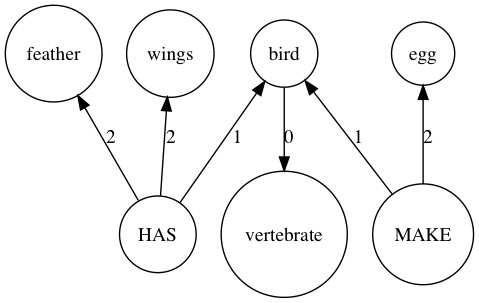
\includegraphics[scale=0.4]{pics/bird.jpg}
\end{figure}
\end{frame}
}
%-----------------------
\begin{frame}
\frametitle{A 4lang szolgáltatás}
		\begin{itemize}
			\pause \item Éles service a \tefl modulra építve
			\pause \item Magasan automatizált gráfgenerálás
			\pause \item Online demo
			\begin{itemize}
				 \item \url{http://4lang.hlt.bme.hu}
			\end{itemize}
			\pause \item Github
			\begin{itemize}
				\item \url{https://github.com/adaamko/4lang}
			\end{itemize}
		\end{itemize}

\end{frame}
%-----------------------
%-----------------------
\begin{frame}
\frametitle{A 4lang szolgáltatás}
\begin{columns}
	\begin{column}{0.4\textwidth}
		I feel bad for my wife!
		\pause 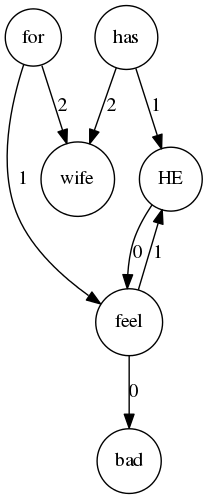
\includegraphics[scale=0.4]{pics/feelbad.png}
	\end{column}
	\begin{column}{0.3\textwidth}
		\pause My poor wife!
		\pause 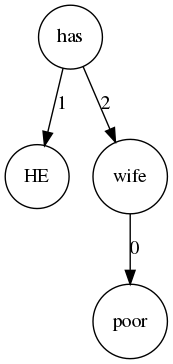
\includegraphics[scale=0.4]{pics/wifepoor.png}
	\end{column}
\end{columns}

\end{frame}
%-----------------------
\begin{frame}
\frametitle{Definiált metrikáink}
\begin{columns}
	\begin{column}{0.5\textwidth}
		\begin{itemize}
			\pause \item \textbf{Cél}
			\begin{itemize}
				\item egy állítás következik-e egy feltevésből?
			\end{itemize}
			\pause \item \textbf{Megvalósítás}
			\begin{itemize}
				\item Gráfok hasonlósága
				\item Mikor hasonló két gráf?
			\end{itemize}
		\end{itemize}
	\end{column}
	\begin{column}{0.5\textwidth}
		\begin{itemize}
			\pause \item My poor wife! (G1)
			\pause \item I feel bad for my wife! (G2)
			\pause \item \[\frac{|E(G_1)\cap E(G_2)|}{|E(G_2)|}\]			
		\end{itemize}
	\end{column}
\end{columns}

\end{frame}
%-----------------------
\begin{frame}
\frametitle{Kiterjesztett gráfok, az "expand" funkció}
\begin{columns}
	\begin{column}{0.1\textwidth}
		\pause 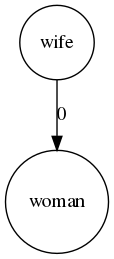
\includegraphics[scale=0.4]{pics/wife.png}
	\end{column}
	\begin{column}{0.1\textwidth}
	\pause \[\Rightarrow\]
	\end{column}
	\begin{column}{0.2\textwidth}
		\pause 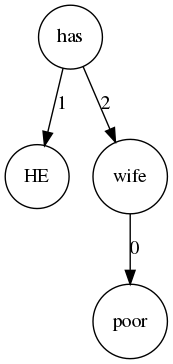
\includegraphics[scale=0.4]{pics/wifepoor.png}
	\end{column}
	\begin{column}{0.1\textwidth}
		\pause \[\Rightarrow\]
	\end{column}
	\begin{column}{0.3\textwidth}
	\pause 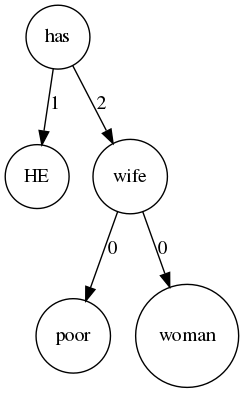
\includegraphics[scale=0.4]{pics/wifeexp.png}
	\end{column}
\end{columns}

\end{frame}


%-----------------------
\begin{frame}
	\frametitle{A gépi szövegértés feladat \citep{Chen:2018, Wang:2018}}
	\begin{columns}
		\begin{column}{0.6\textwidth}
			\begin{itemize}
				\pause \item \textbf{2018-as Semeval Task}
				\begin{itemize}
					\item \textit{Machine comprehension using commonsense knowledge}
				\end{itemize}
				\pause \item Rövid szövegekből egyszerű feleletválasztós kérdések
			\end{itemize}
		\end{column}
		\begin{column}{0.5\textwidth}
			\begin{itemize}
			\pause \item Két legjobb rendszer
			\begin{itemize}
				\item \texttt{HFL-RC}
				\item \texttt{Yuanfudao}
			\end{itemize}
			\pause \item \textbf{MCScript}
			\begin{itemize}
				\item tanító és teszt adat
			\end{itemize}
		\end{itemize}
		\end{column}
	\end{columns}
	
	\end{frame}
%-----------------------
\begin{frame}
    \frametitle{Baseline}
    \begin{figure}
        \centering
        \small
            \begin{itemize}
				\item Minden kérdés válasz párhoz mergelt gráf
				\item A "jobban" hasonló lesz a helyes válasz
				\item \textbf{68,3} accuracy score
			\end{itemize}
            \begin{columns}
				\begin{column}{0.2\textwidth}
					\pause 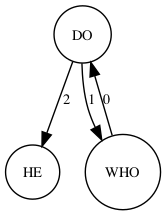
\includegraphics[scale=0.5]{pics/didit.png}
				\end{column}
				\begin{column}{0.2\textwidth}
				\pause \[\Rightarrow\]
				\end{column}
				\begin{column}{0.2\textwidth}
					\pause 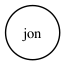
\includegraphics[scale=0.5]{pics/jon.png}
				\end{column}
				\begin{column}{0.2\textwidth}
					\pause \[\Rightarrow\]
				\end{column}
				\begin{column}{0.3\textwidth}
				\pause 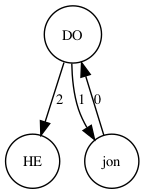
\includegraphics[scale=0.5]{pics/jondid.png}
				\end{column}
			\end{columns}
        \label{fig:method}
        \end{figure}
\end{frame}
%-----------------------

\begin{frame}
\frametitle{Összefoglalás}
\begin{itemize}
    \pause \item Automatizált módszer és metrikák hasonlóság mérésére.
    \pause \item Erős baseline a gépi szövegértés feladatra
    \pause \item Baseline módszerunk alkalmazása state-of-the-art rendszerben, kis javulást hozva
    \pause \item A kód elérhető \url{https://github.com/adaamko/4lang}
    \pause \item Éles Rest API és online demo \url{http://4lang.hlt.bme.hu}
\end{itemize}

\end{frame}
%-----------------------
%-----------------------
\begin{frame}
    \frametitle{Köszönjük!}
    \AtNextBibliography{\tiny}
    \printbibliography
\end{frame}
%-----------------------



\end{document}






